\section{The Implementation: The Search Process}
\label{sec:pit}

Now that we have discussed all the theoretical components of the search engine, it is time to move on to the actual implementation. In this section we describe in detail how a search query is processed and how it is presented to the end user.

\subsection{Entering A Query}

As to give an overview of what exactly happens during a typical search, we will show what happens during a normal search process. From the user perspective, everything happens inside a web browser. When the user visits the demo page \cite{self:sqesdemo}, they are presented with a frontend as shown in Figure \ref{fig:frontmain}.

\begin{figure}[h]
  \begin{center}
    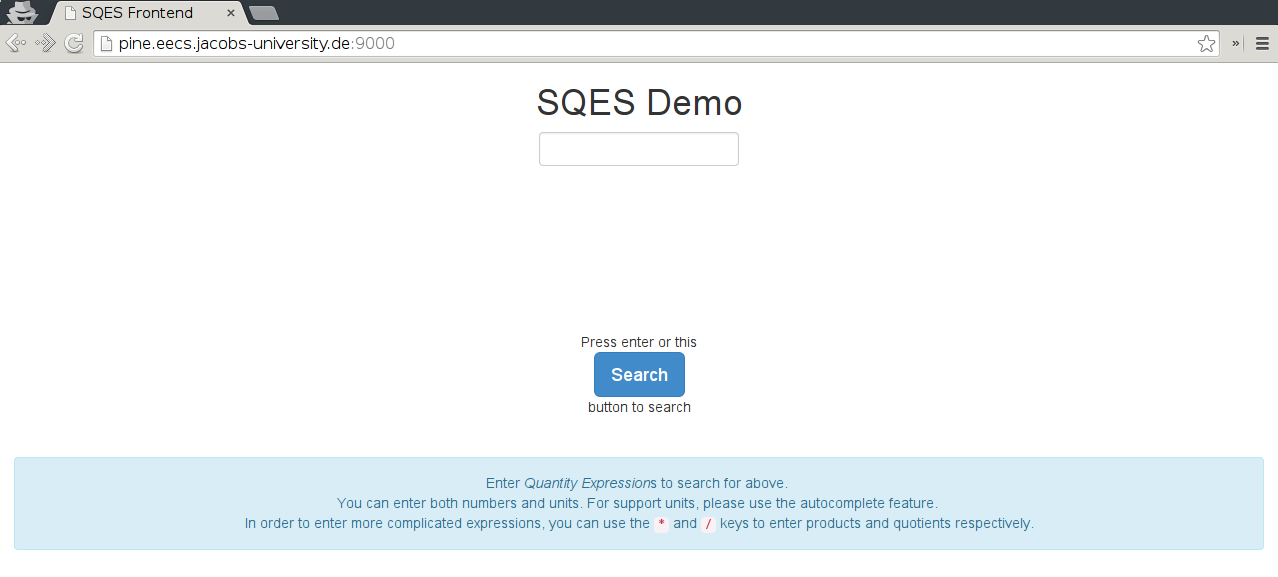
\includegraphics[width=100mm]{img/screen1.png}
  \end{center}
  \caption{The main page of the frontend. }
  \label{fig:frontmain}
\end{figure}

Because the frontend is running inside a Webbrowser it is written using HTML, CSS and JavaScript. Furthermore it uses the frameworks jQuery \cite{lib:jquery} and Bootstrap \cite{lib:bootstrap}. As seen in the figure, the main components are a text field to enter a quantity expression as well as a search button.

With the text field it is easily possible to enter composed quantity expression.

When searching for a certain unit it is neccessary to tell the backend which \textit{unit theory} this unit comes from. In order to make this easier, the GUI has an autocompletion feature. It is only required to enter the name of the unit itself and the possible theories this unit can come from will be suggested automatically.

Apart from entering a simple unit it is possible for the user to compose quantity expressions by multiplication and division. If the keys ``*'' and ``/'' are pressed, the text field splits into two different fields. In each of them another quantity expression can be entered.

In order to facilitate entering division and multiplication by numbers, it is also possible to enter numbers into these fields. With this input unit it is also possible to enter all the quantity expressions as described by the formalism above. In Figure \ref{fig:frontauto} the process of entering the query $42 \frac{\text{Furlong}}{\text{Fortnight}}$ is shown.

\begin{figure}
  \centering
  \begin{subfigure}[b]{0.9\textwidth}
          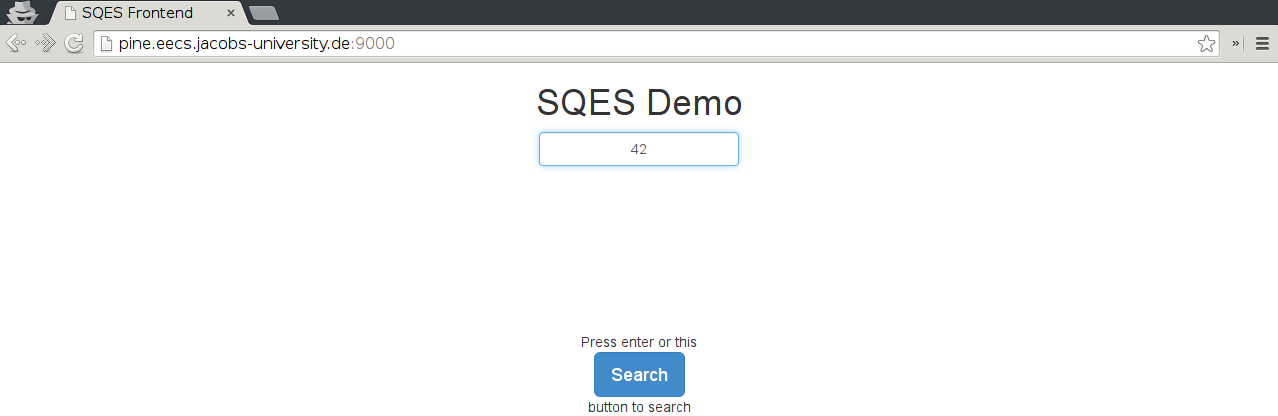
\includegraphics[width=\textwidth]{img/enter1}
          \caption{Entering a number}
          \label{fig:frontauto1}
  \end{subfigure}
  \\
  \begin{subfigure}[b]{0.9\textwidth}
          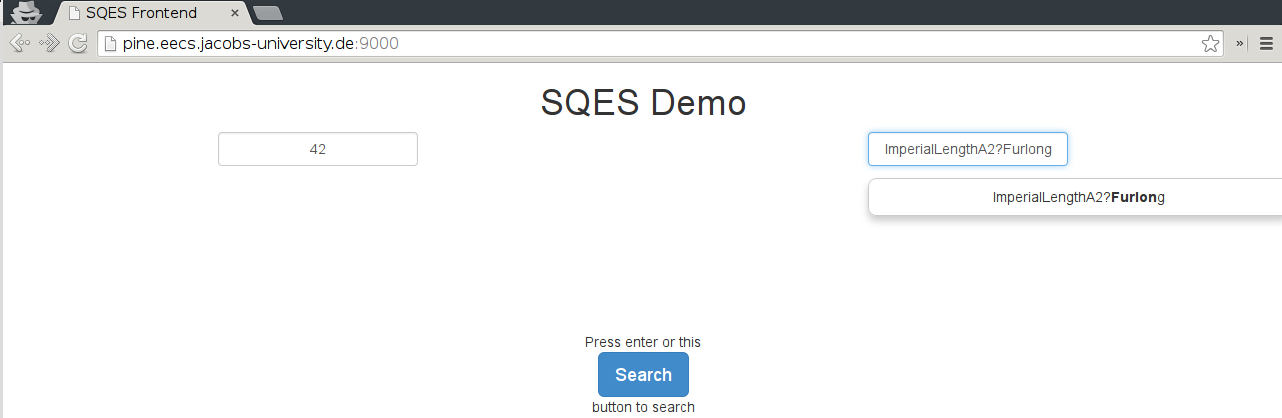
\includegraphics[width=\textwidth]{img/enter2}
          \caption{Entering and autocompleting the unit \textit{Furlong}}
          \label{fig:frontauto2}
  \end{subfigure}
  \\
  \begin{subfigure}[b]{0.9\textwidth}
          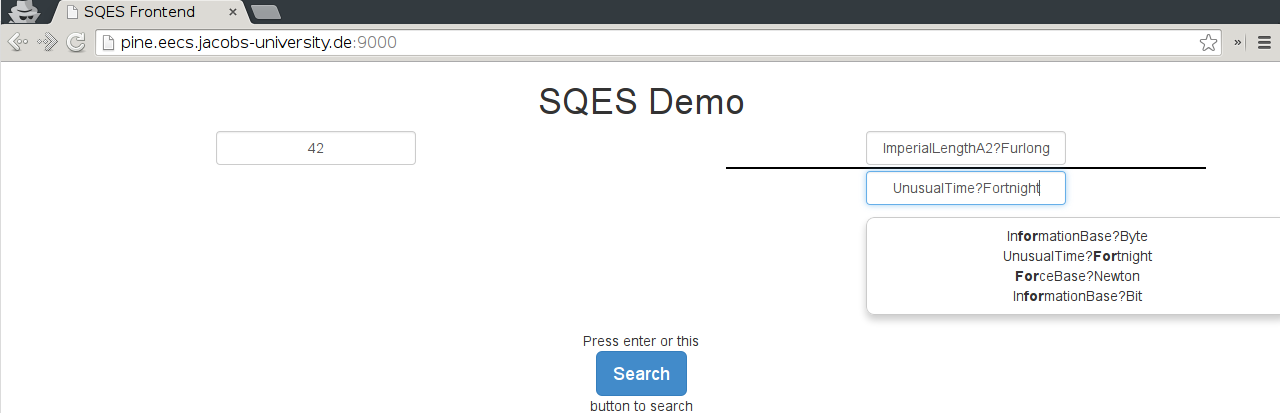
\includegraphics[width=\textwidth]{img/enter3}
          \caption{Entering the final component. }
          \label{fig:frontauto3}
  \end{subfigure}
  \caption{Process of entering the quantity expression $42 \frac{\text{Furlong}}{\text{Fortnight}}$ into the frontend. }
  \label{fig:frontauto}
\end{figure}

\subsection{Processing A Typical Query}

After the quantity expression has been entered, the search can be started by pressing the \textit{Search} button or hitting the \textit{Enter} key. The query inputted into the text field is then serialised to XML as shown in Section \ref{sec:xml}.



\subsection{Presenting The Results}
